\documentclass{beamer}

% --- Pacotes essenciais (seguros com o tema SINTEF) ---
\usepackage[T1]{fontenc}
\usepackage[utf8]{inputenc} % remova se compilar com XeLaTeX/LuaLaTeX
\usepackage[portuguese]{babel}
\usepackage{lmodern}
\usepackage{amsmath,amsfonts}
\usepackage{oldgerm} % você já usava; pode remover se não precisar

% --- Tema e fontes ---
\usetheme{sintef}
\usefonttheme[onlymath]{serif}

% --- Macros do seu template/exemplos ---
\newcommand{\testcolor}[1]{\colorbox{#1}{\textcolor{#1}{test}}~\texttt{#1}}
\newcommand{\hrefcol}[2]{\textcolor{cyan}{\href{#1}{#2}}}

% --- Title background (versão estrelada, antes do \maketitle) ---
\titlebackground*{assets/background}

% --- Bibliografia: mostrar número do item ---
\setbeamertemplate{bibliography item}{\insertbiblabel}

% --- Metadados ---
\title{Attention Models: da motivação às variantes modernas}
\subtitle{Intuição geométrica, formulação matemática e aplicações}
\author{Seu Nome}
\date{\today}

\begin{document}

\maketitle

% ============================
% Evolução: LSTM → Atenção → Transformer (apenas frames)
% ============================

\section{Evolução: LSTM \texorpdfstring{$\rightarrow$}{->} Atenção \texorpdfstring{$\rightarrow$}{->} Transformer}


\begin{frame}{Redes Neurais Recorrentes}
	\framesubtitle{Motivação}

	\begin{figure}[h]
		\centering
		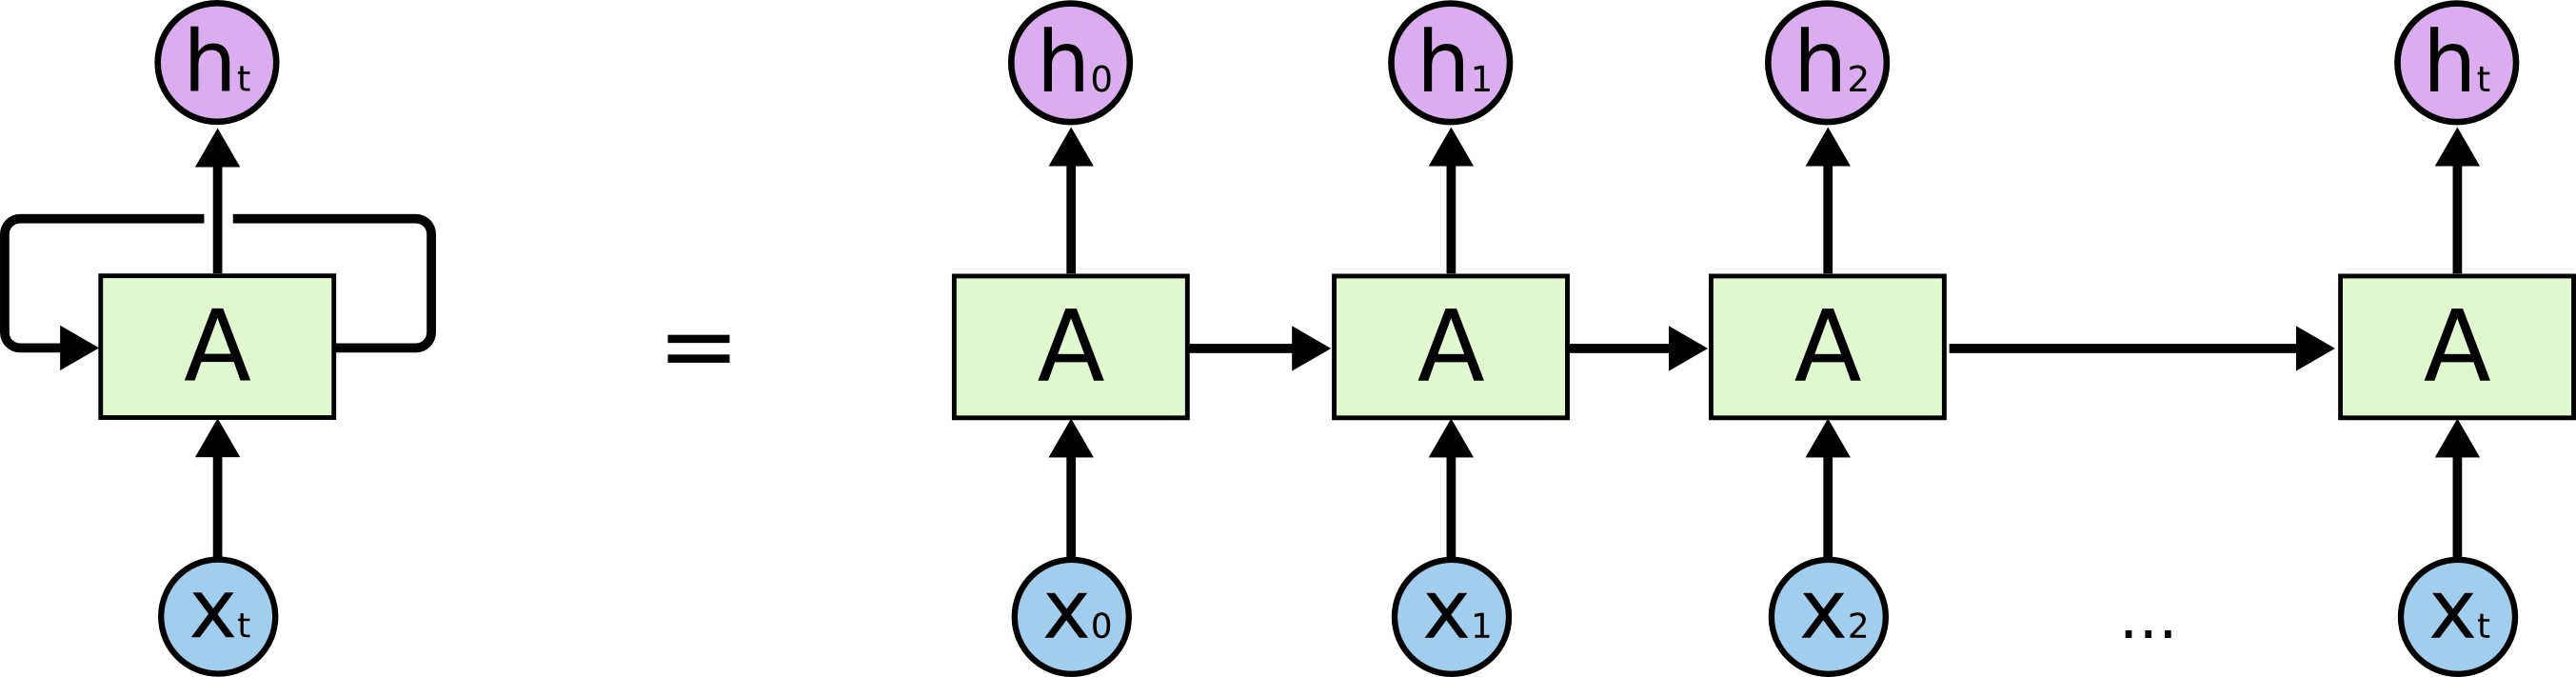
\includegraphics[width=0.6\textwidth]{assets/colah-RNN-unrolled.png}
		\caption{Redes Neurais Recorrentes \footnote{Figura de \href{https://colah.github.io/posts/2015-08-Understanding-LSTMs/}{Christopher Olah}}}
	\end{figure}

	\begin{itemize}
		\item Bem adaptadas para dados sequenciais como séries temporais e texto
		\item Diferentes tipos de modelos: LSTM, GRU
		\item Diferentes arquiteturas: simples, bidirecional, encoder-decoder
	\end{itemize}

\end{frame}

\begin{frame}{Tipos de camadas RNN}
	\framesubtitle{Motivação}
	\begin{columns}[t]
		\column{0.5\textwidth}
		\begin{center}
			\textbf{LSTM}
		\end{center}

		\begin{figure}[h]
			\centering
			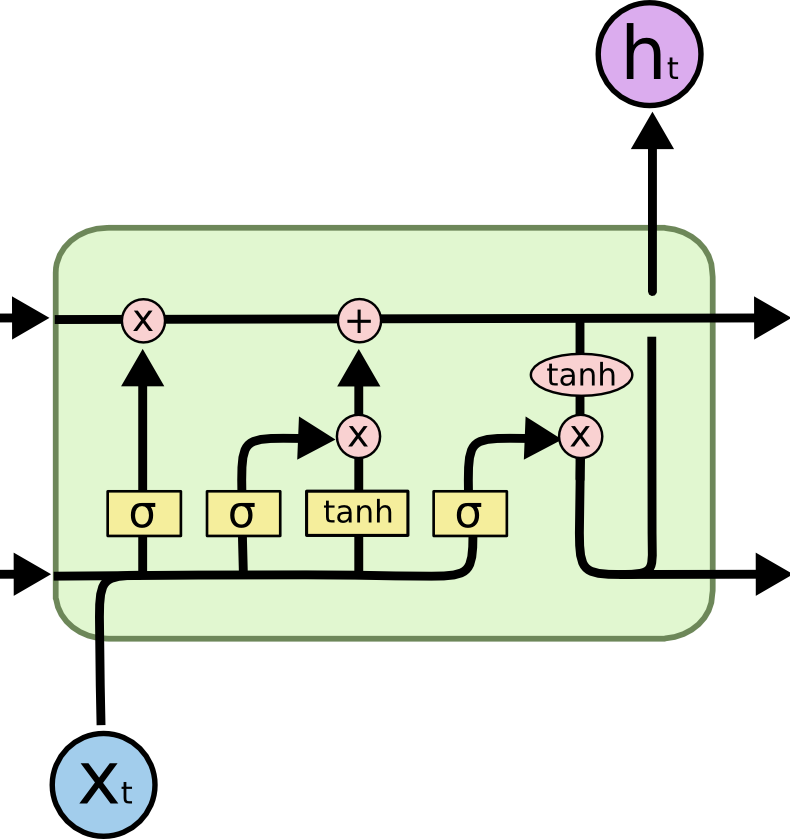
\includegraphics[width=0.33\textwidth]{assets/colah-LSTM-layer.png}
		\end{figure}

		\tiny\[
			\begin{aligned}
				f_t         & = \sigma(W_f \cdot \left[h_{t-1}, x_t \right] + b_f) \\
				i_t         & = \sigma(W_i \cdot \left[h_{t-1}, x_t \right] + b_i) \\
				\tilde{C}_t & = \tanh(W_c \cdot \left[h_{t-1}, x_t \right] + b_c)  \\
				C_t         & = f_t \odot C_{t-1} + i_t \odot \tilde{C}_t          \\
				o_t         & = \sigma(W_o \cdot \left[h_{t-1}, x_t \right] + b_o) \\
				h_t         & = o_t \odot \tanh(c_t)
			\end{aligned}
		\]
		\column{0.5\textwidth}
		\begin{center}
			\textbf{GRU}
		\end{center}

		\begin{figure}[h]
			\centering
			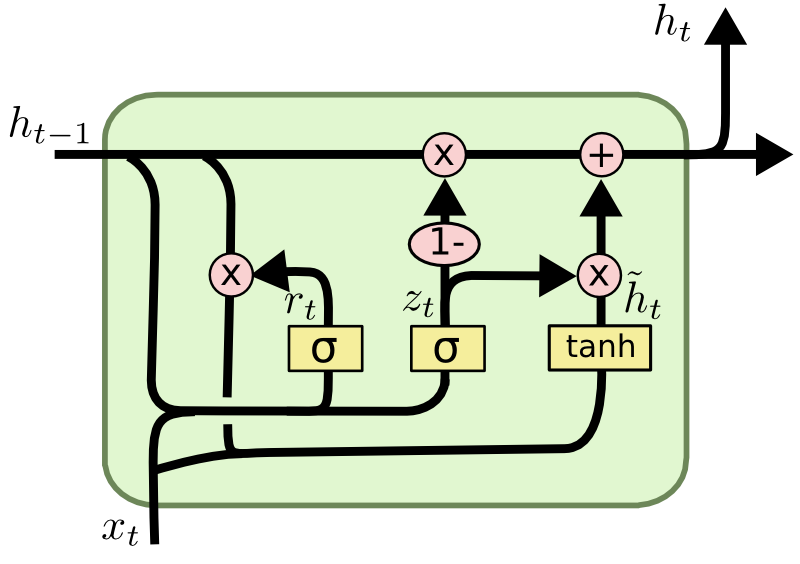
\includegraphics[width=0.33\textwidth]{assets/colah-GRU-layer.png}
		\end{figure}

		\tiny\[
			\begin{aligned}
				z_t         & = \sigma(W_z \cdot \left[h_{t-1}, x_t \right])        \\
				r_t         & = \sigma(W_r \cdot \left[h_{t-1}, x_t \right])        \\
				\tilde{h}_t & = \tanh(W \cdot \left[r_t \odot h_{t-1}, x_t \right]) \\
				h_t         & = (1 - z_t) \odot h_{t-1} + z_t \odot \tilde{h}_t
			\end{aligned}
		\]

	\end{columns}
\end{frame}

% 1) LSTM baseline: encoder-decoder e gargalo
\begin{frame}{LSTM como baseline para NMT}
	\begin{itemize}
		\item Encoder LSTM lê $(x_1,\dots,x_n)$ e produz estados $h_t$; o contexto é o último estado $c=h_n$.
		\item Decoder LSTM gera $(y_1,\dots,y_m)$ condicionado a $c$.
	\end{itemize}
	\[
		\begin{aligned}
			i_t & = \sigma(W_i x_t + U_i h_{t-1} + b_i),\quad
			f_t = \sigma(W_f x_t + U_f h_{t-1} + b_f),              \\
			o_t & = \sigma(W_o x_t + U_o h_{t-1} + b_o),\quad
			\tilde{c}_t = \tanh(W_c x_t + U_c h_{t-1} + b_c),       \\
			c_t & = f_t \odot c_{t-1} + i_t \odot \tilde{c}_t,\quad
			h_t = o_t \odot \tanh(c_t).
		\end{aligned}
	\]
	\begin{itemize}
		\item \textbf{Gargalo}: toda a informação comprimida em $c=h_n$.
	\end{itemize}
\end{frame}

% 2) Limitações do LSTM
\begin{frame}{Limitações do LSTM (motivação para atenção)}
	\begin{itemize}
		\item Processamento \textbf{sequencial} $\Rightarrow$ baixa paralelização.
		\item \textbf{Dependências longas} ainda são difíceis (mesmo com portas).
		\item \textbf{Gargalo do contexto} (vetor único) degrada qualidade em frases longas.
	\end{itemize}
\end{frame}

% 3) Solução 1: Atenção sobre o encoder (Bahdanau/Luong)
\begin{frame}{Atenção no encoder--decoder (Bahdanau/Luong)}
	\textbf{Atenção aditiva (Bahdanau):}
	\[
		e_{ij} = v^\top \tanh\!\big(W_1 h_i + W_2 s_j\big),\quad
		\alpha_{ij} = \mathrm{softmax}_i(e_{ij}),\quad
		c_j = \sum_i \alpha_{ij} h_i .
	\]
	\textbf{Atenção multiplicativa (Luong):}
	\[
		e_{ij} = s_j^\top W h_i \quad \text{(general)}, \qquad
		e_{ij} = s_j^\top h_i \quad \text{(dot)}.
	\]
	\begin{itemize}
		\item Para gerar $y_j$, o decoder combina todos os $h_i$ via pesos $\alpha_{ij}$ (alinhamento dinâmico).
		\item \textbf{Resolve o gargalo}, melhora frases longas e dá interpretabilidade (mapas de atenção).
		\item Ainda há recursão no decoder (processo sequencial).
	\end{itemize}
\end{frame}

% 4) Solução 2: Self-Attention (intra-sequência)
\begin{frame}{Self-Attention: dependências em paralelo}
	\[
		\mathrm{Att}(Q,K,V)=\mathrm{softmax}\!\left(\frac{QK^\top}{\sqrt{d_k}}\right)V,
		\quad
		Q = XW_Q,\; K = XW_K,\; V = XW_V.
	\]
	\begin{itemize}
		\item Calcula relações \emph{entre todos os tokens} da mesma sequência, \textbf{em paralelo}.
		\item Multi-head:
		      \[
			      \mathrm{MHA}(X)=\mathrm{Concat}(H_1,\dots,H_h)\,W_O,\quad
			      H_r=\mathrm{softmax}\!\left(\frac{Q_r K_r^\top}{\sqrt{d_k}}\right)V_r.
		      \]
		\item Comparativo: RNN/LSTM exige $n$ passos sequenciais; self-attention faz um passo paralelo com custo $\mathcal{O}(n^2)$.
	\end{itemize}
\end{frame}

% 5) Transformer: tirar LSTM, adicionar posição + FFN e empilhar blocos
\begin{frame}{Attention Is All You Need: nascendo o Transformer}
	\begin{itemize}
		\item \textbf{Remove} completamente a recorrência (sem LSTM).
		\item \textbf{Positional encodings} preservam ordem:
		      \[
			      PE_{(pos,2i)}=\sin\!\left(\frac{pos}{10000^{2i/d_{\text{model}}}}\right),\quad
			      PE_{(pos,2i+1)}=\cos\!\left(\frac{pos}{10000^{2i/d_{\text{model}}}}\right).
		      \]
		\item Cada \textbf{bloco Transformer} (pré-norm, forma comum):
		      \[
			      \begin{aligned}
				      Y & = X + \mathrm{MHA}(\mathrm{LN}(X)),                                               \\
				      Z & = Y + \mathrm{FFN}(\mathrm{LN}(Y)),\quad \mathrm{FFN}(u)=W_2\,\phi(W_1u+b_1)+b_2,
			      \end{aligned}
		      \]
		\item Empilha-se vários blocos de atenção+FFN $\Rightarrow$ \textbf{arquitetura Transformer}.
	\end{itemize}
\end{frame}

% 6) Máscara causal e síntese da evolução
\begin{frame}{Máscara causal e síntese da evolução}
	\textbf{Máscara causal} (para LMs) impede olhar o futuro:
	\[
		\mathrm{softmax}\!\left(\frac{QK^\top}{\sqrt{d_k}}+M\right),
		\quad
		M_{ij}=\begin{cases}
			0,       & j\le i \\
			-\infty, & j>i
		\end{cases}
	\]
	\textbf{Linha do tempo (síntese):}
	\begin{itemize}
		\item LSTM encoder--decoder: contexto único $c=h_n$ (gargalo).
		\item LSTM + \textbf{atenção} (Bahdanau/Luong): alívio do gargalo.
		\item \textbf{Self-attention}: dependências longas em paralelo.
		\item \textbf{Transformer}: atenção + posição + FFN; várias camadas empilhadas; sem LSTM.
	\end{itemize}
\end{frame}

%===========================
% ROADMAP
%===========================
\section{Roteiro}
\begin{frame}{Roteiro da Apresentação}
	\begin{itemize}[<+->]
		\item Motivação e histórico
		\item Modelos de sequência (RNN/LSTM) + Attention
		\item Embeddings, interpretação geométrica e matemática
		\item Transformers e posicionais
		\item Aplicações: Séries Temporais, Language Models, ViT, GAT
		\item Treinamento, variantes e hiperparâmetros
		\item Tamanho ideal (scaling), Mixture of Experts
		\item Pruning e Distillation
		\item Limitações, diagnóstico e conclusões
	\end{itemize}
\end{frame}

%===========================
% MOTIVAÇÃO & HISTÓRICO
%===========================
\begin{chapter}[assets/background_negative]{sintefdarkgreen}{Motivação \& Histórico}\end{chapter}

\section{Motivação}
\begin{frame}{Por que Atenção?}
	\begin{itemize}[<+->]
		\item Capturar dependências longas e filtrar informação relevante
		\item RNNs sofrem com gradientes e paralelização limitada
		\item Pesos de atenção ajudam na interpretabilidade
		\item Melhor relação capacidade/compute em diversas tarefas
	\end{itemize}
\end{frame}

\begin{frame}{Histórico em 3 passos}
	\begin{itemize}[<+->]
		\item \textbf{Additive Attention} (Bahdanau) para NMT
		\item \textbf{Dot-Product Attention} (Luong) — caminho para escalabilidade
		\item \textbf{Transformers} (Vaswani et al., 2017): “Attention is All You Need”
	\end{itemize}
\end{frame}

%===========================
% FUNDAMENTOS
%===========================
\begin{chapter}[assets/background_negative]{sintefgreen}{Fundamentos}\end{chapter}

\section{Modelos de Sequência}
\begin{frame}{RNN/GRU/LSTM — limites práticos}
	\begin{itemize}[<+->]
		\item Cálculo sequencial $\Rightarrow$ baixa paralelização
		\item Dependências longas: vanish/explode (mitigado, não resolvido)
		\item Memória finita e custo de treino elevado para contextos longos
	\end{itemize}
\end{frame}

\begin{frame}{LSTM + Attention (Encoder--Decoder)}
	\framesubtitle{Atenção aditiva (Bahdanau)}
	\begin{block}{Equações}
		\small
		\[
			e_{ij} = v^\top \tanh\!\big(W_1\,h_i + W_2\,s_j\big), \quad
			\alpha_{ij} = \mathrm{softmax}_i(e_{ij}), \quad
			c_j = \sum_i \alpha_{ij} h_i
		\]
	\end{block}
	\begin{itemize}[<+->]
		\item \textbf{Alinhamento} dinâmico entre estados do encoder e passos do decoder
		\item Reduz gargalos de um único vetor de contexto
	\end{itemize}
\end{frame}

\section{Embeddings \& Interpretações}
\begin{frame}{Word/Subword Embeddings}
	\begin{itemize}[<+->]
		\item Estáticos (Word2Vec, GloVe) vs. Contextuais (ELMo, BERT)
		\item Subword (BPE/Unigram) para robustez morfológica
		\item Análogos em outras modalidades: patches (ViT), time2vec (TS), node2vec (grafos)
	\end{itemize}
\end{frame}

\begin{frame}{Interpretação Geométrica da Atenção}
	\begin{itemize}[<+->]
		\item $Q,K,V$ são projeções lineares do latente
		\item Similaridade (coseno/dot) guia uma \emph{combinação convexa} de $V$
		\item Multi-head $\Rightarrow$ múltiplas métricas/projeções simultâneas
	\end{itemize}
\end{frame}

\begin{frame}{Interpretação Matemática: Self-Attention}
	\begin{block}{Fórmula central (scaled dot-product)}
		\[
			\mathrm{Att}(Q,K,V) \;=\; \mathrm{softmax}\!\left(\frac{QK^\top}{\sqrt{d_k}}\right)\,V
		\]
	\end{block}
	\begin{itemize}[<+->]
		\item Máscara causal/atencional conforme a tarefa
		\item Complexidade $\mathcal{O}(n^2)$ em tempo/memória
		\item Gradientes e saturação da softmax
	\end{itemize}
\end{frame}

\begin{frame}{Positional Encodings}
	\begin{itemize}[<+->]
		\item Absolutos senoidais vs. aprendidos
		\item Relativos e RoPE (rotary): melhor generalização/composição
		\item Impacto em extrapolação e contextos longos
	\end{itemize}
\end{frame}

%===========================
% TRANSFORMERS
%===========================
\begin{chapter}[assets/background_negative]{sinteflightgreen}{Transformers}\end{chapter}

\section{Arquiteturas \& Variantes}
\begin{frame}{Arquiteturas Transformer}
	\begin{itemize}[<+->]
		\item \textbf{Encoder--Decoder}, \textbf{Encoder-only}, \textbf{Decoder-only}
		\item Bloco: MHSA + FFN, \textit{residual} + \textit{layer norm}
		\item Pré-norm vs. pós-norm (estabilidade de treino)
	\end{itemize}
\end{frame}

\begin{frame}{Atenções Eficientes}
	\begin{itemize}[<+->]
		\item \textbf{Esparsidade}: Longformer/BigBird (padrões locais+globais)
		\item \textbf{Aproximação}: Linformer, Nyströmformer
		\item \textbf{Kernels}: Performer (favor+), FlashAttention (IO-aware)
		\item \textbf{Outros}: Reformer (LSH)
	\end{itemize}
	\begin{block}{Trade-off}
		Complexidade $\mathcal{O}(n^2)$ $\rightarrow$ $\tilde{\mathcal{O}}(n)$ com perda controlada de exatidão e/ou restrições de padrão.
	\end{block}
\end{frame}

\section{Treino \& Hiperparâmetros}
\begin{frame}{Práticas de Treino}
	\begin{itemize}[<+->]
		\item AdamW, warmup + decaimento; label smoothing quando aplicável
		\item Regularização: dropout, stochastic depth, weight decay
		\item AMP/mixed precision, grad clipping, checkpointing
		\item Dados: curriculum, masking, augmentation (TS/ViT/GAT)
	\end{itemize}
\end{frame}

\begin{frame}{Hiperparâmetros Essenciais}
	\begin{itemize}[<+->]
		\item Profundidade, $d_{\text{model}}$, \#heads, $d_{ff}$, dropout
		\item Comprimento de contexto, batch size, \textit{LR schedule}
		\item Específicos: tokenização (LM), \textit{patch size} (ViT), janela/patch (TS)
	\end{itemize}
\end{frame}

\begin{frame}{Qual tamanho ideal? (Scaling)}
	\begin{itemize}[<+->]
		\item Leis de escala vs. limite de dados/compute
		\item Tokens vs. parâmetros; saturação com contexto
		\item Regra prática: dimensione para o dataset e o \textit{budget} de inferência
	\end{itemize}
\end{frame}

%===========================
% APLICAÇÕES
%===========================
\begin{chapter}[assets/background_negative]{sintefyellow}{Aplicações}\end{chapter}

\section{Séries Temporais}
\begin{frame}{Atenção em Séries Temporais}
	\begin{itemize}[<+->]
		\item Codificação temporal: absolutos/relativos, time2vec, calendários/sazonalidade
		\item Exógenas e \textit{cross-attention}; \textit{patching} para contextos longos
		\item Tarefas: previsão, imputação, detecção de anomalias
	\end{itemize}
\end{frame}

\section{Language Models}
\begin{frame}{Language Models (LM)}
	\begin{itemize}[<+->]
		\item Atenção \textbf{causal}, \textit{next-token} e \textit{masking}
		\item Pré-treino vs. \textit{fine-tuning}; Instrução/LoRA/Adapters
		\item Métricas: perplexidade e tarefas \textit{downstream}
	\end{itemize}
\end{frame}

\section{Vision Transformer}
\begin{frame}{Vision Transformer (ViT)}
	\begin{itemize}[<+->]
		\item Imagem $\rightarrow$ \textit{patches} + \texttt{[CLS]} token
		\item Posicionais 2D; augmentations (RandAug, Mixup/CutMix)
		\item Transfer: \textit{linear probe} vs. \textit{fine-tune}
	\end{itemize}
\end{frame}

\section{Graph Attention}
\begin{frame}{Graph Attention Networks (GAT)}
	\begin{block}{Coeficientes de Atenção (um cabeçalho)}
		\small
		\[
			\alpha_{ij}=\mathrm{softmax}_j\!\left(\mathrm{LeakyReLU}\!\big(a^\top[Wh_i \,||\, Wh_j]\big)\right)
		\]
	\end{block}
	\begin{itemize}[<+->]
		\item Multi-head; sobre-\textit{smoothing} e escalabilidade
		\item Heterógrafos e atenção relacional
	\end{itemize}
\end{frame}

%===========================
% ESCALA & COMPRESSÃO
%===========================
\begin{chapter}[assets/background_negative]{sintefred}{Escala \& Compressão}\end{chapter}

\section{MoE, Pruning, Distillation}
\begin{frame}{Mixture of Experts (MoE)}
	\begin{itemize}[<+->]
		\item \textit{Gating} top-1/top-2; balanceamento de carga
		\item Roteamento esparso: capacidade vs. ociosidade
		\item Custos de comunicação e estabilidade no treino
	\end{itemize}
\end{frame}

\begin{frame}{Pruning}
	\begin{itemize}[<+->]
		\item Não estruturado (magnitude) vs. estruturado (canal/bloco, n:m)
		\item Iterativo vs. \textit{one-shot}; impacto em latência real
		\item Interação com quantização e \textit{sparsity-aware kernels}
	\end{itemize}
\end{frame}

\begin{frame}{Distillation}
	\begin{block}{Perda típica (Hinton)}
		\small
		\[
			\mathcal{L}=(1-\lambda)\,\mathrm{CE}(y,s)+\lambda\,T^2\,\mathrm{KL}\!\big(p_T \,\|\, q_T\big)
		\]
	\end{block}
	\begin{itemize}[<+->]
		\item \textit{Teacher} $\rightarrow$ \textit{student}; temperatura $T$
		\item \textit{Intermediate layer hints}; \textit{task-specific} vs. generalista
		\item Benefícios: latência/energia e \textit{edge deployment}
	\end{itemize}
\end{frame}

%===========================
% INTERPRETAÇÃO & LIMITES
%===========================
\begin{chapter}[assets/background_negative]{sinteflilla}{Interpretação \& Limitações}\end{chapter}

\section{Diagnóstico \& Limites}
\begin{frame}{Interpretação \& Diagnóstico}
	\begin{itemize}[<+->]
		\item \textit{Attention rollout/flow}; atenção $\neq$ causalidade
		\item \textit{Probing} de camadas; ablação de cabeças
		\item Ferramentas de \textit{explainability} por domínio
	\end{itemize}
\end{frame}

\begin{frame}{Limitações \& Trade-offs}
	\begin{itemize}[<+->]
		\item Custo $\mathcal{O}(n^2)$, viés de dados, \textit{OOD} robustness
		\item Contaminação de treino e privacidade
		\item Energia/carbono e restrições de hardware
	\end{itemize}
\end{frame}

%===========================
% CONCLUSÕES
%===========================
\section{Conclusões}
\begin{frame}{Conclusões}
	\begin{itemize}[<+->]
		\item Atenção como princípio unificador em sequência, visão e grafos
		\item Escolha guiada por dados, métricas e orçamento (treino/inferência)
		\item Escala e compressão (MoE/pruning/distillation) para produção
	\end{itemize}
\end{frame}

%===========================
% Q&A
%===========================
\backmatter
\begin{frame}
	\frametitle{Perguntas?}
	\centering
	Obrigado!
\end{frame}

%===========================
% BACKUP (opc.)
%===========================
\section{Backup (Opcional)}
\begin{frame}{Equações úteis (resumo)}
	\small
	\begin{itemize}
		\item Scaled dot-product, aditiva (Bahdanau)
		\item Atenção relativa e RoPE
		\item GAT detalhado; máscaras causais
	\end{itemize}
\end{frame}

\begin{frame}{Hiperparâmetros por tarefa (resumo)}
	\small
	\begin{itemize}
		\item LM: contexto, BPE, heads/profundidade típicos
		\item ViT: patch size, MLP ratio, augmentations
		\item TS: janela, patching, covariáveis, perdas (MAE/MSE/Quantile)
	\end{itemize}
\end{frame}

%===========================
% REFERÊNCIAS
%===========================
\section{Referências Bibliográficas}
\begin{frame}[allowframebreaks]
	\frametitle{Referências Bibliográficas}
	\bibliographystyle{ieeetr}
	\bibliography{presentation_bib.bib}
\end{frame}

\end{document}
